\documentclass[tikz,border=5pt]{standalone}
\usetikzlibrary{spath3}
\begin{document}
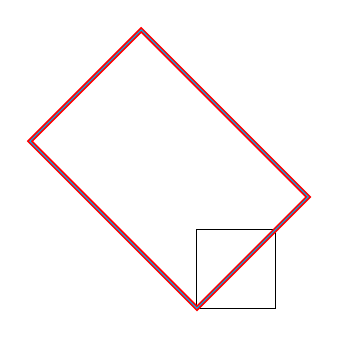
\begin{tikzpicture}
    \draw[spath/save=tpath] (0,0) rectangle +(1,1); 
    \draw[rotate=45, xscale=2, yscale=3, ultra thick, red] (0,0) rectangle +(1,1); 
    \draw[
        cyan,spath/transform={tpath}{rotate=45, xscale=2, yscale=3},spath/use={tpath}
    ]; % 实现相同的路径变换效果
\end{tikzpicture}

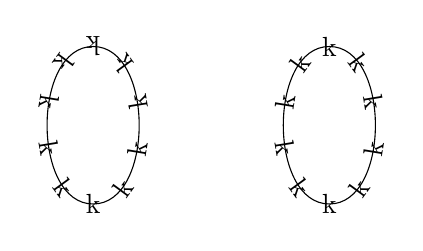
\begin{tikzpicture}
    \draw[spath/save=oval] (0,0) 
    to[out=0,in=0] (0,2)
    to[out=180,in=180] (0,0); 
    \foreach \k in {0,...,9} {
        \node[
            transform shape, 
            spath/transform to={oval}{0.\k}
        ] {k};
    }
    \begin{scope}[xshift = 3cm]
        \draw[spath/save=soval] (0,0) 
        to[out=0,in=0] (0,2)
        to[out=180,in=180] (0,0); 
        \foreach \k in {0,...,9} {
            \node[
                transform shape, 
                spath/upright transform to={soval}{0.\k}]
            {k};
        }
    \end{scope} 
\end{tikzpicture}

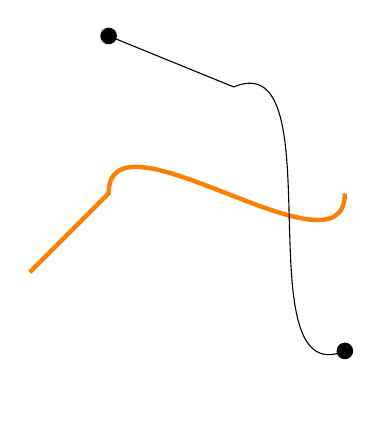
\begin{tikzpicture}
    \path[draw=orange,ultra thick,spath/save=a] 
    (3,2) -- ++(1,1) to[out=90,in=-90] ++(3,0);
    \tikzset{ spath/span={a}{(4,5)}{(7,1)}} % 路径变换
    \fill (4,5) circle[radius=3pt] (7,1) circle[radius=3pt];
    \draw[spath/use=a]; 
\end{tikzpicture}
\end{document}